\documentclass[12pt,a4paper]{article}

\usepackage[T1]{fontenc}
\usepackage[utf8]{inputenc}
\usepackage{newtxtext}
\usepackage{newtxmath}
\usepackage{amsmath}
\usepackage{amsfonts}
\usepackage{amssymb}
\usepackage{graphicx}
\usepackage{tikz}
\usetikzlibrary{arrows.meta, positioning, shapes.geometric}
\usepackage{hyperref}
\usepackage{geometry}
\usepackage{setspace}
\usepackage{fancyhdr}
\usepackage{booktabs}
\usepackage{tabularx}
\usepackage{array}
\usepackage{float}
\usepackage{enumitem}
\usepackage{caption}

\geometry{
\ta4paper,
\tleft=20mm,
\tright=20mm,
\ttop=20mm,
\tbottom=25mm,
}

\raggedbottom
\setstretch{1.15}
\setlength{\parindent}{1.25em}
\setlength{\parskip}{0.2em}
\setlength{\tabcolsep}{8pt}
\renewcommand{\arraystretch}{1.15}
\setlength{\headheight}{15pt}
\setlist[itemize]{itemsep=0.25em, topsep=0.35em, leftmargin=1.5em}
\setlist[enumerate]{itemsep=0.25em, topsep=0.35em, leftmargin=1.5em}
\setlength{\textfloatsep}{10pt plus 2pt minus 2pt}
\setlength{\intextsep}{10pt plus 2pt minus 2pt}
\setlength{\abovecaptionskip}{4pt}
\setlength{\belowcaptionskip}{2pt}
\captionsetup{font=small,labelfont=bf,skip=4pt}

\pagestyle{fancy}
\fancyhf{}
\fancyhead[L]{}
\fancyhead[C]{Project Report}
\fancyhead[R]{}
\fancyfoot[C]{\thepage}
\renewcommand{\headrulewidth}{0.4pt}
\renewcommand{\footrulewidth}{0pt}

\hypersetup{
\tcolorlinks=true,
\tlinkcolor=black,
\turlcolor=blue,
\tcitecolor=black
}

\newcolumntype{Y}{>{\raggedright\arraybackslash}X}
\newcolumntype{L}[1]{>{\raggedright\arraybackslash}p{#1}}

\begin{document}

\pagenumbering{roman}
\tableofcontents
\newpage
\listoffigures
\newpage
\pagenumbering{arabic}

\section{Introduction}
Traffic Racer is a Unity-based arcade driving project built around a simple but repeatable gameplay loop. The player moves from the Main Menu to the Garage, selects a vehicle, and then enters the SampleScene to dodge traffic on an endless road. The project is intentionally modular so that menu flow, car selection, vehicle physics, traffic spawning, and user feedback can be developed and tested independently.

\subsection{Problem Statement}
Arcade racing games often become difficult to maintain when scene transitions, vehicle logic, and UI code are mixed together. That makes it harder to extend the project with new cars, new scenes, or new feedback systems. This project addresses that problem by separating the game into a small set of focused Unity scripts that coordinate scene flow, player setup, traffic generation, and end-of-run presentation.

\subsection{Objectives}
The main objectives of the project are:
\begin{itemize}
    \item Build a playable endless driving game with responsive keyboard controls.
    \item Provide a clear scene flow from the Main Menu to the Garage and then to gameplay.
    \item Support car selection and preserve that choice across scene transitions.
    \item Generate traffic dynamically so each run feels slightly different.
    \item Present speed, distance, score, and game-over information through the UI.
    \item Keep the implementation understandable enough for course evaluation and future extension.
\end{itemize}

\subsection{Development Environment \& Tools}
\begin{table}[!htbp]
\centering
\caption{Development Environment and Primary Tools}
\begin{tabularx}{\textwidth}{@{}L{4.2cm}Y@{}}
\toprule
Component & Purpose \\
\midrule
Unity Editor 6000.3.9f1 & Primary game engine, scene editor, physics runtime, and build pipeline. \\
C\# & Main scripting language used for gameplay logic and scene coordination. \\
Visual Studio Code / Visual Studio & Source editing and debugging. \\
Git and GitHub & Version control and collaboration. \\
TextMesh Pro & High-quality text rendering for the HUD and results panel. \\
LeanTween asset package & Available in the project assets for tweening support; some UI motion is also implemented with coroutines. \\
Unity built-in physics and audio systems & Vehicle physics, collisions, audio playback, and scene management. \\
\bottomrule
\end{tabularx}
\end{table}

\subsection{Methodology and Design Approach}
The project uses a scene-based design. Menu and garage logic remain in their own scenes, while gameplay logic lives in SampleScene. Shared state such as the selected car is stored in lightweight runtime data and PlayerPrefs so the chosen vehicle can be restored after a scene change. This approach keeps each script narrow in scope and reduces hard dependencies between UI, audio, camera, and gameplay systems.

\section{Project Overview}

\subsection{Gameplay Concept}
The game is built around a straightforward endless-driving concept. The player drives forward through traffic, avoids collisions, and tries to survive for as long as possible while the HUD continuously updates run statistics. The pace of the game is intentionally easy to understand: choose a car, start the run, steer through traffic, and restart after a crash.

\subsection{Key Features}
\begin{itemize}
    \item Scene-based navigation between the Main Menu, Garage, and SampleScene.
    \item Vehicle preview and selection in the Garage scene.
    \item Player car persistence across scenes through runtime state and PlayerPrefs.
    \item Wheel-collider-based vehicle movement, steering, and braking.
    \item Random traffic spawning with lane-based placement.
    \item Endless road and city recycling to simulate continuous forward motion.
    \item HUD feedback for speed, distance, score, and game-over summary.
    \item Scene-specific audio for menus, gameplay, and UI actions.
\end{itemize}

\subsection{Intended Users and Use Cases}
The intended audience is an undergraduate course evaluator and casual players who want a short arcade-style driving experience. Typical use cases include opening the game from the menu, selecting a preferred vehicle, entering gameplay, attempting a longer run, and returning to the menu or restarting after a collision.

\section{Game Flow and System Architecture}
This section summarizes the full player journey and the main system boundaries. Figure~\ref{fig:scene-flow} shows the end-to-end flow from launch to gameplay and back to the menu, while Figure~\ref{fig:architecture} shows how the main scripts are grouped around the scene structure.

\subsection{Whole-Game Flowchart}
\begin{figure}[!htbp]
\centering
\resizebox{0.98\textwidth}{!}{%
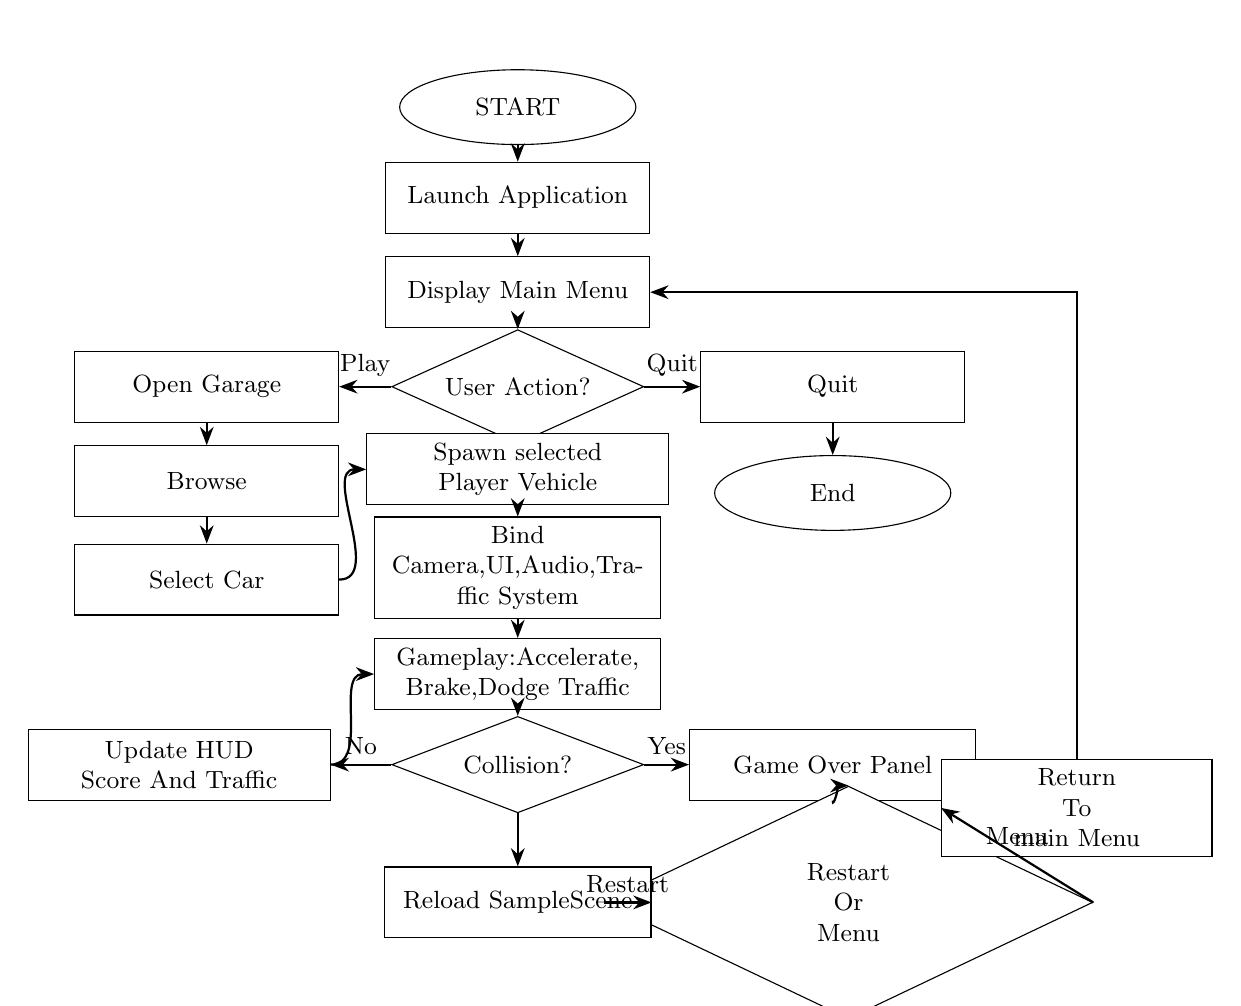
\begin{tikzpicture}[
    >=Stealth,
    font=\small,
    term/.style={ellipse, draw, minimum width=3.0cm, minimum height=0.95cm, align=center, fill=white},
    process/.style={rectangle, draw, minimum width=3.35cm, minimum height=0.9cm, align=center, fill=white},
    decision/.style={diamond, draw, aspect=2.1, minimum width=3.2cm, minimum height=1.15cm, align=center, fill=white},
    arrow/.style={-Stealth, thick}
]
\node[term] (start) at (0,0) {START};
\node[process] (launch) at (0,-1.15) {Launch Application};
\node[process] (menu) at (0,-2.35) {Display Main Menu};
\node[decision] (action) at (0,-3.55) {User Action?};

\node[process] (garage) at (-3.95,-3.55) {Open Garage};
\node[process] (browse) at (-3.95,-4.75) {Browse};
\node[process] (selectcar) at (-3.95,-6.0) {Select Car};

\node[process, text width=3.6cm] (spawn) at (0.0,-4.6) {Spawn selected\\Player Vehicle};
\node[process, text width=3.4cm] (bind) at (0.0,-5.85) {Bind\\Camera,UI,Audio,Tra-\\ffic System};
\node[process, text width=3.4cm] (gameplay) at (0.0,-7.2) {Gameplay:Accelerate,\\Brake,Dodge Traffic};
\node[decision] (collision) at (0.0,-8.35) {Collision?};

\node[process, text width=3.6cm] (update) at (-4.3,-8.35) {Update HUD\\Score And Traffic};
\node[process, text width=3.4cm] (gameover) at (4.0,-8.35) {Game Over Panel};
\node[decision, text width=3.4cm] (restartmenu) at (4.2,-10.1) {Restart\\Or\\Menu};
\node[process, text width=3.15cm] (reload) at (0.0,-10.1) {Reload SampleScene};
\node[process, text width=3.2cm] (returnmenu) at (7.1,-8.9) {Return\\To\\main Menu};
\node[process, text width=2.8cm] (quit) at (4.0,-3.55) {Quit};
\node[term] (end) at (4.0,-4.9) {End};

\draw[arrow] (start) -- (launch);
\draw[arrow] (launch) -- (menu);
\draw[arrow] (menu) -- (action);
\draw[arrow] (action.west) -- node[above] {Play} (garage.east);
\draw[arrow] (action.east) -- node[above] {Quit} (quit.west);
\draw[arrow] (quit) -- (end);

\draw[arrow] (garage) -- (browse);
\draw[arrow] (browse) -- (selectcar);
\draw[arrow] (selectcar.east) to[out=0,in=180] (spawn.west);

\draw[arrow] (spawn) -- (bind);
\draw[arrow] (bind) -- (gameplay);
\draw[arrow] (gameplay) -- (collision);
\draw[arrow] (collision.west) -- node[above] {No} (update.east);
\draw[arrow] (collision.south) -- (reload.north);
\draw[arrow] (update.east) to[out=0,in=180] (gameplay.west);
\draw[arrow] (collision.east) -- node[above] {Yes} (gameover.west);
\draw[arrow] (gameover.south) to[out=-90,in=180] (restartmenu.north);
\draw[arrow] (restartmenu.west) -- node[above] {Restart} (reload.east);
\draw[arrow] (restartmenu.east) -- node[above] {Menu} (returnmenu.west);
\draw[arrow] (returnmenu.north) |- (menu.east);
\end{tikzpicture}%
}
\caption{Whole-game scene transition flowchart}
\label{fig:scene-flow}
\end{figure}

The flowchart shows that the game has a predictable progression: launch, menu, car selection, gameplay, collision handling, and return paths for either restart or menu navigation. This structure is important for an undergraduate project because it makes the overall behavior easy to explain and easy to test.

\subsection{System Architecture Overview}
\begin{figure}[!htbp]
\centering
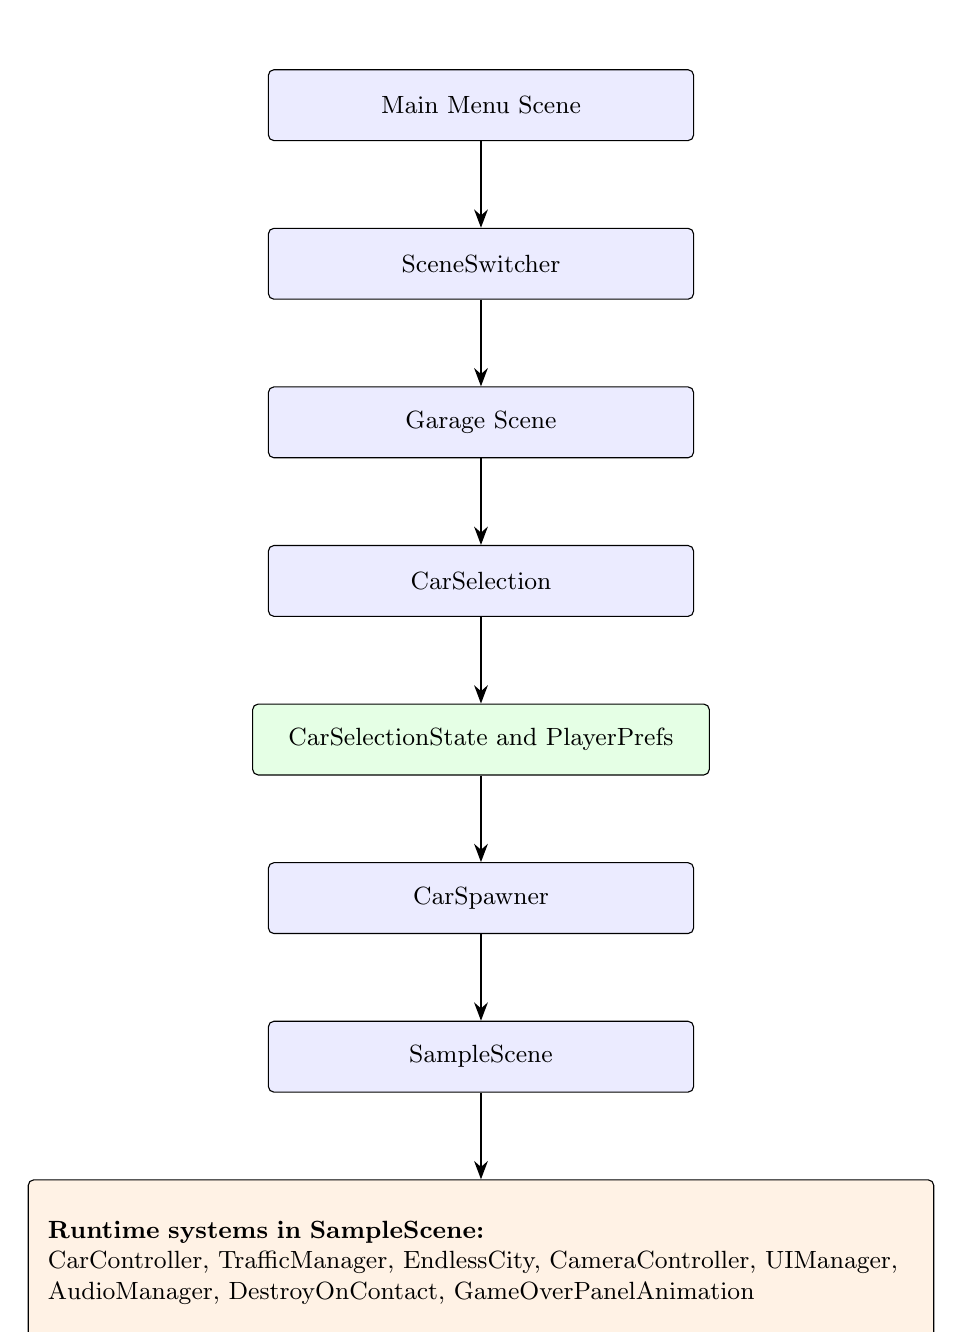
\begin{tikzpicture}[
    node distance=1.1cm,
    >=Stealth,
    font=\small,
    box/.style={rectangle, draw, rounded corners=2pt, minimum width=5.4cm, minimum height=0.9cm, align=center, fill=blue!8},
    state/.style={rectangle, draw, rounded corners=2pt, minimum width=5.8cm, minimum height=0.9cm, align=center, fill=green!10},
    runtime/.style={rectangle, draw, rounded corners=2pt, text width=11cm, minimum width=11.5cm, minimum height=2.1cm, align=left, fill=orange!10},
    arrow/.style={-Stealth, thick}
]
\node[box] (mainmenu) {Main Menu Scene};
\node[box, below=of mainmenu] (switcher) {SceneSwitcher};
\node[box, below=of switcher] (garage) {Garage Scene};
\node[box, below=of garage] (selection) {CarSelection};
\node[state, below=of selection] (persist) {CarSelectionState and PlayerPrefs};
\node[box, below=of persist] (spawner) {CarSpawner};
\node[box, below=of spawner] (sample) {SampleScene};
\node[runtime, below=of sample] (runtime) {\textbf{Runtime systems in SampleScene:}\\CarController, TrafficManager, EndlessCity, CameraController, UIManager, AudioManager, DestroyOnContact, GameOverPanelAnimation};

\draw[arrow] (mainmenu) -- (switcher);
\draw[arrow] (switcher) -- (garage);
\draw[arrow] (garage) -- (selection);
\draw[arrow] (selection) -- (persist);
\draw[arrow] (persist) -- (spawner);
\draw[arrow] (spawner) -- (sample);
\draw[arrow] (sample) -- (runtime);
\end{tikzpicture}
\caption{High-level system architecture}
\label{fig:architecture}
\end{figure}

The architecture diagram shows a clean boundary between scene transitions and runtime gameplay. Menu and garage scripts focus on presentation and selection, while the gameplay scene contains the vehicle, traffic, camera, UI, audio, and collision systems that run during active play.

\section{Codebase Structure}
The repository follows the standard Unity layout, with the majority of project-specific logic concentrated in \texttt{Assets/Scripts}. Scenes, prefabs, and asset folders are separated so that the report can describe the project in terms of responsibility rather than file noise.

\subsection{Directory Layout}
\begin{itemize}
    \item \texttt{Assets/Scenes/} contains the scene files for the Main Menu, Garage, and SampleScene.
    \item \texttt{Assets/Scripts/} contains the gameplay, UI, audio, selection, and camera scripts.
    \item \texttt{Assets/Prefabs/} stores reusable player cars, traffic objects, and related scene objects.
    \item \texttt{Assets/Materials/}, \texttt{Assets/Animation/}, and \texttt{Assets/Car Game Sound Effects/} provide the visual and audio resources used by the scenes.
    \item \texttt{Assets/LeanTween/} is included as a tweening asset package in the project tree.
    \item \texttt{Packages/} and \texttt{ProjectSettings/} contain Unity package and project configuration data.
\end{itemize}

\subsection{Core Scripts and Responsibilities}
\begin{table}[!htbp]
\centering
\caption{Core Scripts and Their Responsibilities}
\begin{tabularx}{\textwidth}{@{}L{4.2cm}Y@{}}
\toprule
Script & Responsibility \\
\midrule
\texttt{CarController.cs} & Handles vehicle input, wheel-collider movement, steering, braking, and collision gating. \\
\texttt{CarSpawner.cs} & Spawns the selected player vehicle in gameplay and reconnects runtime systems to the new car. \\
\texttt{CarSelection.cs} & Manages garage navigation, selected-car persistence, and loading of SampleScene. \\
\texttt{CarSelectionState.cs} & Stores the current selected car index, name, and identifier in static runtime state. \\
\texttt{TrafficManager.cs} & Spawns traffic vehicles at random lanes with timing influenced by player speed. \\
\texttt{EndlessCity.cs} & Recycles city segments to create the appearance of an endless route. \\
\texttt{UIManager.cs} & Updates the speed, distance, score, and game-over interface. \\
\texttt{AudioManager.cs} & Provides singleton music and sound-effect control across scenes. \\
\texttt{SceneSwitcher.cs} & Handles fade-based scene transitions and button-triggered navigation. \\
\texttt{CameraController.cs} & Keeps the camera following the player smoothly during gameplay. \\
\texttt{DestroyOnContact.cs} & Removes traffic objects that are no longer needed after a contact event. \\
\texttt{GameOverPanelAnimation.cs} & Adds a small scale-in animation to the results panel. \\
\bottomrule
\end{tabularx}
\end{table}

\subsection{Major Data Structures}
\begin{table}[!htbp]
\centering
\caption{Important Runtime Data Structures}
\begin{tabularx}{\textwidth}{@{}L{4.1cm}Y@{}}
\toprule
Structure & Use \\
\midrule
\texttt{CarSelectionState} static fields & Preserve the selected car index, identifier, and name after scene changes. \\
\texttt{PlayerPrefs} keys such as \texttt{CarIndexValue} and \texttt{SelectedCarId} & Persist the selected vehicle between runs and across sessions. \\
\texttt{WheelCollider} references in \texttt{CarController} & Provide physically-based wheel movement, steering, and braking. \\
\texttt{Transform[]} lane arrays in \texttt{TrafficManager} & Define the valid spawn positions for traffic vehicles. \\
\texttt{GameObject[]} traffic prefabs & Hold the pool of available traffic vehicle models. \\
\texttt{TextMeshProUGUI} references in \texttt{UIManager} & Bind the HUD and game-over text fields to the scene UI. \\
\texttt{AudioSource} references in \texttt{AudioManager} & Separate music playback from button sound playback. \\
\bottomrule
\end{tabularx}
\end{table}

\subsection{Key Function Prototypes}
\begin{table}[!htbp]
\centering
\caption{Key Function Prototypes and Roles}
\begin{tabularx}{\textwidth}{@{}L{4.4cm}Y@{}}
\toprule
Function & Role \\
\midrule
\texttt{CarController.FixedUpdate()} & Reads input and applies torque, steering, braking, and wheel updates. \\
\texttt{CarController.HandleVehicleImpact()} & Filters valid traffic collisions and triggers the crash flow only when needed. \\
\texttt{CarSpawner.SpawnCar()} & Resolves the selected vehicle, instantiates it, and rebinds gameplay systems. \\
\texttt{CarSelection.StartGameFromGarage()} & Saves the selected car and loads SampleScene. \\
\texttt{TrafficManager.SpawnTraffic()} & Continuously creates traffic vehicles after a short delay. \\
\texttt{EndlessCity.Update()} & Repositions road or city segments once the player crosses the threshold. \\
\texttt{UIManager.Update()} & Refreshes the HUD values during active gameplay. \\
\texttt{UIManager.GameOver()} & Freezes the game, shows end-of-run results, and hides the live HUD. \\
\texttt{SceneSwitcher.cs: SceneLoaderWithSound()} & Plays button audio and performs the fade-based scene transition. \\
\texttt{AudioManager.PlayMenuMusic()} and \texttt{PlayGameMusic()} & Switch the active music track based on the current scene. \\
\bottomrule
\end{tabularx}
\end{table}

\subsection{External Libraries and Dependencies}
\begin{table}[!htbp]
\centering
\caption{External Libraries and Dependencies}
\begin{tabularx}{\textwidth}{@{}L{4.2cm}Y@{}}
\toprule
Dependency & Use \\
\midrule
UnityEngine scene, physics, and audio modules & Core gameplay runtime, collisions, vehicle motion, and scene loading. \\
TextMesh Pro & Crisp and scalable interface text. \\
LeanTween asset folder & Included as a reusable tweening library in the project assets. \\
Unity standard UI system & Buttons, panels, Canvas groups, and HUD elements. \\
\bottomrule
\end{tabularx}
\end{table}

\section{Implementation Details}

\subsection{Core Procedure}
The gameplay loop follows a fixed sequence. The player opens the Main Menu, moves to the Garage to choose a car, and then enters SampleScene. During scene initialization, \texttt{CarSpawner.cs} rebuilds the selected vehicle and reconnects the dependent systems. Once the run starts, \texttt{CarController.cs} handles input and vehicle motion, \texttt{TrafficManager.cs} spawns traffic obstacles, \texttt{EndlessCity.cs} recycles the environment, \texttt{CameraController.cs} follows the player, and \texttt{UIManager.cs} refreshes the HUD. If a valid collision occurs, the game switches to the Game Over state and offers either a restart or a return to the Main Menu.

\subsection{Scene Initialization and Car Selection}
The player starts in the Main Menu and can move into the Garage through a fade-based transition. \texttt{CarSelection.cs} resets the scene time scale, restores audio playback, and displays the last selected car. When the player changes the selection, the script updates the current index, stores the selected car identifier and name, and saves the values using PlayerPrefs. This makes the garage behave like a persistent selection screen rather than a temporary preview.

When SampleScene begins, \texttt{CarSpawner.cs} resolves the selected vehicle from either the current runtime state or the saved PlayerPrefs values. It then instantiates the correct player prefab, ensures a \texttt{CarController} is available, attaches or configures \texttt{CarSound}, and rebinds the camera, UI, traffic, and road scripts to the spawned car. That runtime rebinding is the main reason the project remains modular: the player car can be replaced without rewriting the rest of the scene logic.

\subsection{Vehicle Physics and Input Handling}
\texttt{CarController.cs} uses WheelCollider components to implement movement. The script reads the horizontal and vertical axes, applies motor torque to the front wheels, adjusts steering angle, and sets brake torque when the space bar is held. The wheel meshes are then updated from the colliders so that the visual model matches the physical state of the car.

The controller also configures the rigidbody center of mass through a dedicated transform, which improves stability during steering and collisions. A short initial impact ignore window is used so the player does not trigger an immediate collision event while the spawned vehicle is still settling into the scene. This small guard makes the gameplay feel more reliable from the first second of each run.

\subsection{Traffic, Road, and Camera Coordination}
Traffic generation is handled by \texttt{TrafficManager.cs}. After a short delay, the script repeatedly spawns traffic vehicles at random lane positions. The delay between spawns decreases as the player's speed increases, which keeps the game pressure consistent as the car moves faster.

The endless driving effect comes from \texttt{EndlessCity.cs}. When the player moves past a threshold, the script relocates the tracked city segment further ahead so the road appears to continue indefinitely. \texttt{CameraController.cs} keeps the view focused on the player by smoothing the camera position toward either a dedicated camera point or a fallback offset attached to the car. Together, these systems create the core illusion of long-distance driving without loading a new level every few seconds.

\subsection{Error Handling and User Feedback}
The HUD is driven by \texttt{UIManager.cs}. Each frame, it reads the player's speed and distance, then converts them into live score text. When the run ends, the script freezes time, shows the game-over panel, and presents the final run statistics. The live HUD icons are hidden at this point so the end screen stays visually clean.

Audio feedback is managed by the singleton \texttt{AudioManager.cs}. It keeps music available across scene changes and switches between menu music and gameplay music when needed. Button presses also play a separate sound effect, which gives menu interactions clear feedback. \texttt{GameOverPanelAnimation.cs} adds a small scale-in animation to the results display so the end screen feels deliberate instead of static.

The scripts also include basic defensive checks to keep the game stable. Null checks are used before reading transforms, UI references, audio clips, and prefabs. \texttt{SceneSwitcher.cs} can still load a scene if the fade CanvasGroup is missing, which prevents a small UI configuration problem from blocking navigation entirely. \texttt{CarSpawner.cs} and \texttt{TrafficManager.cs} log useful errors when required prefabs or references are not assigned, and \texttt{DestroyOnContact.cs} filters non-traffic objects so it does not delete unrelated scene objects by mistake.

\section{Usage Examples}
A typical play session follows this sequence:
\begin{enumerate}
    \item Open the Main Menu and choose the Garage option.
    \item Browse the available cars and confirm the desired selection.
    \item Start SampleScene and wait for the player car to spawn.
    \item Drive with the keyboard, avoid traffic, and monitor the HUD.
    \item After a collision, review the results panel and either restart or return to the menu.
\end{enumerate}

For development and demonstration purposes, the game can also be launched directly from the Unity Editor by opening \texttt{Assets/Scenes/MainMenu.unity} and pressing Play. That workflow is useful when checking scene transitions, audio states, or car selection behavior during debugging.

\section{Testing \& Results}
\subsection{Testing Approach}
The project should be validated through manual playtesting in the Unity Editor and in the packaged build. The main checks focus on scene navigation, car selection persistence, traffic spawning, camera stability, UI updates, collision handling, and the return path to the menu after game over. Because this is an undergraduate project, the emphasis is placed on observable behavior rather than on a large automated test suite.

\subsection{Test Scenarios and Observed Results}
\begin{table}[!htbp]
\centering
\caption{Test Scenarios and Validation Checklist}
\begin{tabularx}{\textwidth}{@{}L{4.1cm}Y Y L{1.4cm}@{}}
\toprule
Scenario & Expected Result & Validation Note & Status \\
\midrule
Main Menu to Garage transition & The garage should open with fade feedback and play the correct scene music. & The garage scene loads correctly and the button audio is triggered. & To verify \\
Car selection and return to gameplay & The selected vehicle should remain active when SampleScene starts. & The chosen car is stored and restored through runtime state and PlayerPrefs. & To verify \\
Traffic spawning during gameplay & Traffic should appear in valid lanes after the initial delay. & Traffic is spawned in random lanes and the timing shortens as speed increases. & To verify \\
Collision with traffic & A valid traffic hit should end the run and show the results panel. & The game-over panel appears and the live HUD is hidden. & To verify \\
Endless road behavior & The road should recycle so the player does not reach a visible end. & The city segment is repositioned when the player crosses the threshold. & To verify \\
Camera follow stability & The camera should remain smoothly aligned with the player car. & The camera follows the car without abrupt jumps during normal play. & To verify \\
\bottomrule
\end{tabularx}
\end{table}

This checklist is sufficient for a small course project because it covers the main systems that shape the player experience. Once the build is exported and exercised on the target machine, the notes in the table can be converted into final observed results if needed.

\section{Limitations \& Future Work}

\subsection{Known Limitations}
\begin{itemize}
    \item The traffic logic is intentionally simple and does not include lane-changing or adaptive AI.
    \item The current control scheme is tuned for keyboard input and desktop play.
    \item The build currently shows run statistics, but a persistent high-score system is not yet finalized in the scripts.
    \item The project uses a modest set of cars and environment assets compared with a full commercial racing title.
\end{itemize}

\subsection{Possible Improvements and Future Work}
The project can be extended in several realistic directions:
\begin{itemize}
    \item Persistent high-score storage and replayable career progression.
    \item Online leaderboards and account-based player profiles.
    \item Multiplayer mode, either local or network-based.
    \item Mobile touch tuning with on-screen buttons, tilt controls, or gesture input.
    \item Controller support and more flexible input presets for different platforms.
    \item Dynamic difficulty scaling so traffic density adapts more smoothly to performance.
    \item More vehicle models, additional roads, and richer environmental variation such as weather or day-night cycles.
    \item Accessibility and settings options such as volume sliders, control remapping, and reduced-motion support.
\end{itemize}

\section{Conclusion}
The Traffic Racer project demonstrates a complete but compact Unity gameplay loop built from a small number of well-defined systems. Scene management, car selection, vehicle physics, traffic spawning, audio, and user feedback are separated into dedicated scripts so the project remains understandable and extensible. For a course submission, the current build is strong enough to show design discipline, working gameplay, and clear opportunities for future expansion.

\end{document}
